\documentclass[10pt,twocolumn]{article}

\usepackage{graphicx}
\usepackage[pagebackref=true, hidelinks]{hyperref}
\usepackage{url}
\usepackage{amsmath}
\usepackage{amssymb}
\usepackage{mathspec}
\usepackage[labelfont={bf,footnotesize,singlespacing},
                textfont={footnotesize,singlespacing},
                justification={justified}]{caption}
\usepackage[round]{natbib}
\bibliographystyle{plainnat}

\usepackage{booktabs}
\usepackage{dcolumn}

\usepackage{nameref}
\usepackage{enumitem}

\usepackage{seqsplit}

\setmainfont[Numbers=OldStyle, Ligatures={TeX}]{Latin Modern Roman}
\AtBeginEnvironment{tabular}{\setmainfont[Numbers={OldStyle,Monospaced}, Ligatures={TeX}]{Latin Modern Roman}}
\newfontfamily\old[Numbers=OldStyle]{Latin Modern Roman}
\usepackage{siunitx}
\sisetup{per-mode = symbol,bracket-unit-denominator = false, mode = text,number-text-rm = \old}
\setmathfont{Latin Modern Math}
\setmathfont(Digits)[Numbers=OldStyle]{Latin Modern Roman}

\usepackage{polyglossia}
\setmainlanguage{english}
\setotherlanguage{greek}

\newfontfamily\greekfont{Latin Modern Math}

\setlength{\columnsep}{0.75cm} % 21.34pt
\usepackage[margin=1.75cm]{geometry} % ~49.79pt
\usepackage{scrextend}

% \usepackage{lineno}
% \linenumbers

\hyphenation{off-chain}
\hyphenation{on-chain}

\title{Pricing liquidity for Lightning wallets}
\author{
	José I. Rojas Echenique\\ \url{jir@galoy.io}
	\and
	Nicolas Burtey\\ \url{nb@galoy.io}
}
\date{March 9, 2022}

\begin{document}
\maketitle

\begin{abstract}

Bitcoin banks that interoperate on the Lightning network
are the most developed path to scaling Bitcoin for mass adoption.
One problem faced by these banks is the implementation
of fees for transactions that incur protocol fees on
the Bitcoin and Lightning networks.
This problem is particularly important in the context of
providing both onchain and offchain liquidity,
since different usage patterns can incur dramatically different protocol fees.
We argue that the possibility of liquidity arbitrage on the Lightning network
sets a market rate for inbound liquidity,
and use an estimate of this market rate to develop new
fee structures that properly price liquidity without overcharging
everyday users.
Furthermore, we perform simulations using
historical transaction data from users of the Bitcoin Beach Wallet,
and show that the new fee structures are able to
account for different usage patterns under realistic conditions.

\end{abstract}

\section{Introduction}

Bitcoin has a fundamental scaling ceiling set by the requirement
for global broadcast and verification of every transaction, onchain.
The Lightning network allows transactions to remain offchain
by allowing users to route bitcoin through onchain-settled payment channels \citep{poon2015}.
Although the Lightning network significantly improves Bitcoin's scalability,
the remaining requirement for onchain transactions to open and close each payment channel,
means that further scaling improvements will be necessary
to accommodate mass adoption \citep{burchert2018}.

Custodial Bitcoin banks, that interoperate on the Lightning network,
could accommodate mass adoption.
Custodial banks allow users to trade-off Bitcoin's
pseudonymous privacy,
permissionlessness, and
censorship resistance
for access to
Bitcoin's open monetary network,
and deflationary monetary policy.
Importantly, this trade-off may be improved in the future
with the development of technologies like
hosted channels with private routing \citep{kumaigorodski2021},
and federated Chaumian mints \citep{sirion2021}.

One challenge faced by custodial Bitcoin banks is the implementation of transaction fees.
Through batching, intelligent liquidity management,
and intraledger transactions, banks can substantially reduce
the fee burden of interacting with the Bitcoin network for their users,
but they can not eliminate it entirely.
To the extent that the bank interfaces with the wider Bitcoin network
it will incur protocol fees that will ultimately have to be paid for by
users of the bank.
Fee structures that account for the real costs of each user's transactions,
would allow banks to be more permissionless,
serving customers with different transactional needs
while staying competitive and sustainable.
This is particularly important in the context of
offering users full liquidity for both onchain and offchain transactions,
where different usage habits can incur dramatically
different protocol fees.

Here, we address the problem of implementing
transaction fees that properly price Lightning liquidity.
We discuss the costs of managing onchain
and offchain liquidity in the Lightning network.
We argue that the possibility of inbound liquidity arbitrage
ensures the emergence of a market rate for inbound liquidity.
Using an estimate of this market rate,
we develop fee structures that account for a
user's transaction history when pricing liquidity.
And finally, we study how these fee structures would impact real users
through simulation, using data from users of the Bitcoin Beach Wallet.

\section{Background}

\subsection{Payment channels and liquidity}

To transact on the Lightning network,
users commit bitcoin to payment channels.
The bitcoin in these channels can be used to
route and send offchain payments but not to transact onchain.
Thus, the user's total balance of bitcoin
will not always be immediately liquid for both onchain and offchain transactions.

The native way of managing onchain and offchain liquidity
on the Lightning network
is by opening and closing payment channels.
To acquire more offchain outbound liquidity,
a user can peg-\emph{in}\footnote{
	Following convention, we use \emph{-in} to refer to transactions
	that move bitcoin into the Lightning network,
	and \emph{-out} to refer to transactions that move bitcoin
	out of the Lightning network.
}
to the Lightning network by opening a channel
between their node and a counterparty's.
Opening a channel requires that a user
commit bitcoin to a 2-of-2 multisignature contract
with a counterparty that is connected to the network and
willing to route the user's payments.
The bitcoin in the new channel is typically provided
entirely by the user that opens the channel,
so the counterparty risks little in accepting.
Moreover, if the user has additional connections to the rest of the network
the counterparty gains inbound liquidity by accepting the channel.
Thus, it is usually easy for users to find willing counterparties.

To acquire more onchain liquidity,
a user can peg-\emph{out} of the Lightning network by closing a channel.
Unlike opening a channel, closing a channel does not require permission
from the counterparty
(though cooperation from the counterparty is preferable,
since, otherwise, the user's bitcoin will be unspendable for length of the lock-time).
In either case, closing a channel reduces the user's \emph{and the counterparty's}
offchain inbound and outbound liquidity.
Thus, unlike opening a channel,
closing a channel negatively impacts the counterparty.

Finally, to acquire more offchain inbound liquidity,
the user needs a peer to commit \emph{their} bitcoin to a new channel
and be willing and able to route payments to the user.
This can happen spontaneously
if the peer expects to be able to collect routing fees from the channel.
Alternatively, users can negotiate reciprocal channel openings
with semi-trusted peers\footnote{
	This can happen
	through informal chat groups like Rings of Fire (\url{https://t.me/theRingsOfFire})
	or PlebNet (\url{https://t.me/plebnet})
	or on platforms designed for the purpose
	like Lightning Network Plus (\url{https://lightningnetwork.plus/}).
},
or pay for inbound liquidity by buying channel leases or committing to dual funded channels
\citep{osuntokun2020, neigut2018}.
In each of these cases, the benefits of the channel for the counterparty must outweigh
the costs of the onchain transaction and capital allocation required to open and maintain the channel.

Two additional operations are in development that would allow users to
manage onchain and offchain liquidity without opening and closing channels.
Channel splicing \citep{russel2018} would allow
users to peg-out by reducing a channel's total capacity
without closing it, thereby maintaining its inbound capacity.
PeerSwap \citep{togami2021} would allow channel partners to trustlessly
swap offchain bitcoin on the channel for onchain bitcoin
and additional inbound capacity.
Both splicing and PeerSwap will reduce the onchain costs of
acquiring inbound liquidity
by allowing users to maintain, or increase, inbound liquidity on existing channels,
rather than always paying the onchain fees for opening new channels.

The different channel operations discussed above
also have second-order effects.
On the Lightning network,
a user's history of channel management operations
is broadcast globally and cryptographically verifiable.
Other users need this information to route payments,
but it may also affect the choices they make
when setting routing fees and choosing potential channel counterparties.
Operations that negatively impact counterparties,
like closing channels or splicing-out,
will negatively affect the user's reputation on the network.
All else being equal,
the profitability of a channel depends on its lifetime \citep{branzei2018}.
Thus, among other considerations,
peers will prefer to open new channels
with users that have a history of long-lived channels
and counterparties will set higher fees to users
that have a history of short-lived channels.

\subsection{Submarine swaps}

The costs of closing channels,
and the challenges of acquiring additional inbound liquidity,
have motivated the development of alternative methods of
managing onchain and offchain liquidity.
``Submarine'' swaps \citep{bosworth2018} are the most widely adopted such alternative.
Swap services,
like Boltz\footnote{\url{https://boltz.exchange/}}
and Loop\footnote{\url{https://Lightning.engineering/loop/}},
operate Lightning network nodes that trustlessly
pay offchain invoices in exchange for onchain bitcoin (swap-in); or
send onchain bitcoin in exchange for offchain payments (swap-out).

Submarine swaps have all the benefits of PeerSwaps with the difference
that the swap is with a central service node rather than a channel counterparty.
This adds a requirement for routing to complete a submarine swap,
which increases the cost of swapping but also provides several benefits.
One is that, by using a multi path payment,
the liquidity on multiple channels can be swapped in a single operation.
Another benefit is that
the routing requirement ensures that the inbound
liquidity gained by swapping-out is fully available to route payments
(at least as far as the swap node).
This dramatically simplifies to process of acquiring inbound liquidity,
since the user no longer needs to determine whether
their counterparty would be willing and able to route their payments
\citep{ZmnSCPxj2020}.

Submarine swaps are trustless and some implementations are open source.
The only barrier to starting a new submarine swap service is
the capital needed to ensure a stock of onchain and offchain liquidity
to offer customers.
This means that there is little to limit competition
driving swap fees to the lowest sustainable rates.
Behind the scenes,
submarine swap services rely on the same native operations of
opening, closing, and acquiring new channels to manage
their onchain and offchain liquidity.\footnote{
	While large swap services may be able to batch
	onchain channel operations more efficiently than users,
	each swap requires an onchain output.
	This requirement limits the extent to which
	large swap services will be able to offer lower
	fees for their service than what the user could
	get by performing the equivalent channel operations.
}
Thus, we can expect that the costs of using
submarine swap services will approach the costs
of the equivalent channel operations,
with additional costs due to the capital allocation
and the need
to route funds to (or from) the service node.
Submarine swaps are useful, not because they reduce fees,
but because they
allow their users to trustlessly out-source
liquidity management channel operations.

Table~\ref{tbl:trustless} shows the swap service fees and
estimated Lightning network routing fees for
swapping-out using Boltz and Loop
(the onchain fee will be roughly
the same for both services and depend on
the current demand for blockspace
rather than the amount swapped).
The two services charge very different fees
but, in practice, the total costs are similar:
Boltz's high swap fees are balanced by Loop's high routing fees.
We can begin to understand the difference between the two services
by noting that Loop's channels are significantly shorter lived
than Boltz' and the rest of the Lightning network's (Figure~\ref{lifetimes}).
Moreover, Loop's high routing fees are not a transient phenomenon;
routing to Loop's node has been consistently more expensive than
the Lightning network average through periods of high and low onchain fees
(Figure~\ref{loop}).
Loop's unique routing characteristics are not unexpected.
Short lived channels with high incoming fees
are one of the costs of managing liquidity through channel operations
and, by providing submarine swaps,
Loop bears this burden in place of the nodes it swaps with.

\begin{table}[tb] \footnotesize
\caption{\label{tbl:trustless}
	Trustless swap-out fees for Loop and Boltz.
	The base and proportional routing fees are estimated from the
	capacity-weighted, median channel fees
	of all open inbound channels on January 31, 2022.
}
\centering
\begin{tabular}{lrr}
\toprule
	&	{Routing (sat, \%)}	&	{Swap (\%)} \\
\midrule
Boltz	&	0.00, 0.01	&	0.5\phantom{*}  \\
Loop	&	1.00, 0.22	&	0.1*	\\
\bottomrule
\end{tabular}
\begin{flushleft}
	* The average fee quoted by the \texttt{loop quote} command
	from October, through December, 2021.
\end{flushleft}
\end{table}

\begin{figure}[tb]
	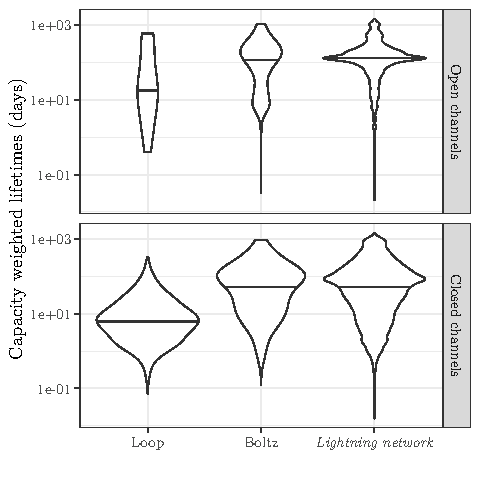
\includegraphics[width=\columnwidth]{fig/routing/lifetimes}
	\caption[Historical channel lifetimes for Loop and Boltz.]{ \label{lifetimes}
		Current (above) and historical (below) channel lifetimes for Loop and Boltz.
		Capacity weighted distributions of lifetimes for channels connected to
		the two submarine swap services, and across the rest of the Lightning network.
		Lines show capacity weighted medians.
		Historical data from \citet{lnchannels}.
	}
\end{figure}

\begin{figure*}[tb]
	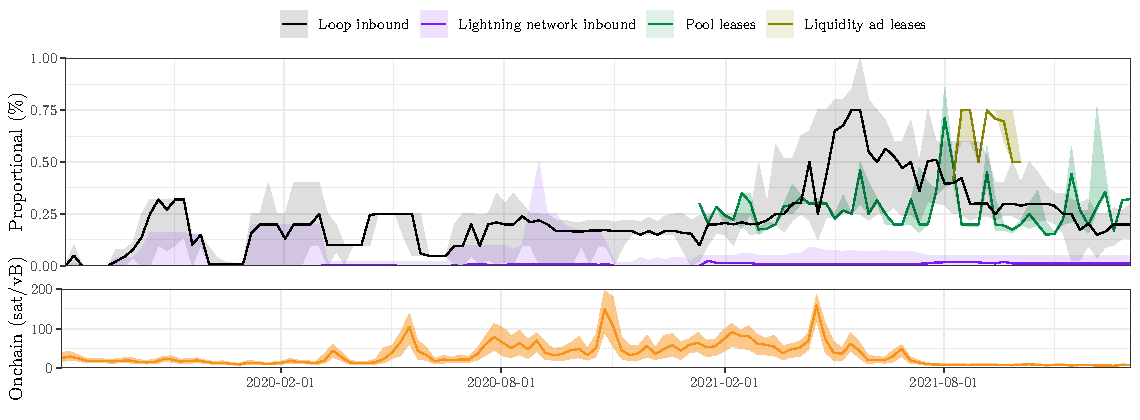
\includegraphics[width=\textwidth]{fig/inbound/inbound}
	\caption[Historical inbound liquidity fees.]{ \label{loop}
		Historical inbound liquidity fees.
		Weekly capacity and duration weighted*
		incoming proportional routing fees for channels
		connected to Loop and the across the rest of the Lightning network
		\citep[data from][]{lnchannels};
		are plotted on the same scale as the node capacity weighted
		proportional fees offered on liquidity ads
		\citep[data from][]{lngossip};
		and the volume weighted cleared proportional fees
		charged by Pool
		\citep[data from][]{poolrates}$\dagger$.
		The lower panel shows onchain fees for comparison.
		Shaded regions show 25\% and 75\% quantiles.
		Data for liquidity ad leases is not plotted where
		historical gossip message archives are unavailable.

		* Since fees can be updated over the course of a channel's
		lifetime, the medians and quantiles are calculated with weights
		determined by the product of the channel's capacity and
		the amount of time between updates.

		$\dagger$ Lease rates for Pool and liquidity ads are not annualized since
		the minimum lease times are sufficient for an inbound liquidity arbitrage.
	}
\end{figure*}

\subsection{Inbound liquidity arbitrage}

To explain Boltz's long channel lifetimes
and low incoming routing fees it suffices to notice that
since Boltz charges a higher swap fee,
it can out-source \emph{its} channel management operations to Loop.
Boltz can keep the routing fees to its node low,
by charging a swap fee that is at least as high as the
sum of the Loop swap fee and routing fees to the Loop node.
Stated another way,
Boltz can outsource its channel operations if
the routing nodes between Boltz and Loop are willing
to sell \emph{their} inbound liquidity to Boltz for, at most,
the difference between the two services' swap fees.
The balance between Boltz's high swap fees and Loop's high routing fees
is maintained by the possibility of arbitrage by routing nodes.

This inbound liquidity arbitrage is a general phenomenon across
the Lightning network.
When any entity offers inbound liquidity at a rate lower than
the routing fees to Loop (or another inbound liquidity sink),
a routing node can profit by acquiring that inbound liquidity and
opening a matching channel to Loop.
This is most clearly illustrated in the market for
inbound channel creation, where the arbitrage is simplest.
Table~\ref{tbl:inbound} shows the channel creation fees
charged by different Lightning network service providers.
The fees are all at least as high as what one could expect
to make by routing to Loop, and the lifetimes are all
sufficient to exhaust a channel's entire capacity
before the channel is closed by Loop (Figure~\ref{lifetimes}).
Figure~\ref{loop} shows the historical fees for inbound channel creation
available on Pool and the liquidity ad market.
During the first half of 2021, it may have been possible for
routing nodes to buy channels from Pool and sell the inbound
liquidity to Loop's customer's at a profit
(though this is uncertain since it's possible that
Pool's service fee was higher during this time).
Since then, the prices for inbound liquidity on Loop and Pool
have reached what appears to be an equilibrium.

\begin{table}[tb] \footnotesize
\caption[Channel creation]{\label{tbl:inbound}
	Lightning service provider fees for inbound channel creation.
	Lifetime refers to the minimum lifetime of the channel,
	it may stay open longer than that.
}
\centering
\begin{tabular}{lrcc}
\toprule
	& {Creation (sat, \%)} & {Lifetime} & Atomic\\
\midrule
Boltz	& 0, 1.50*	& --- & yes \\
LNBIG	& 4500, 0.21$\dagger$	& 1 month & no \\
lnd-routing	& 500, 0.25\phantom{*}	& 1 month & no \\
Liquidity ads	& 612, 0.42$\ddagger$	& 1 month & yes \\
Pool	& 0, 0.25\S	& \S & yes \\
Thor	& 10,425, 1.11\phantom{*}	& 1 month & no \\
\bottomrule
\end{tabular}
\begin{flushleft}

	* Boltz charges a 0.5\% fee for swapping-in,
	if the user does not have enough inbound capacity to receive
	the swapped-in funds, Boltz creates a channel with
	an additional capacity of 25\% inbound liquidity.

	$\dagger$ This fee does not include the cost of the
	channel creation transaction.


	$\ddagger$ Node-capacity-weighted medians calculated on
	February 16, 2022.  Does not include the cost of the
	channel creation transaction.

	\S\, In addition to this fee, Pool charges a service fee of 0.05\% - 0.25\%;
	half of the channel creating transaction fee;
	and a, one time, 1,000 satoshi flat fee.
	Channel lifetimes are enforced onchain and available for
	2, 4, or 12 weeks or 1 year.

\end{flushleft}
\end{table}

Another way of acquiring additional inbound liquidity is by
trading-out using custodial services,
that allow both onchain and offchain deposits and withdrawals.
Since selling inbound liquidity is not the primary purpose of these services,
it may be possible to find conditions under which acquiring inbound liquidity
using a custodial service is cheaper in terms of fees than
using a trustless swap service.
Table~\ref{tbl:custodial} shows estimates for the routing fees associated
with depositing offchain bitcoin to several custodial services
as well as the service fees for onchain withdrawals and a summary
of KYC requirements for each service.
When compared to Tables~\ref{tbl:trustless}~and~\ref{tbl:inbound}, it is clear that
some of these custodial services offer much cheaper inbound liquidity than
other services.
For many routing node operators,
this could represent an attractive arbitrage opportunity.
On the other hand, using a custodial service comes with additional costs and limitations, such as:
custody risk;
privacy;
deposit, withdraw, and balance limits;
and terms of use restrictions.
Moreover, since custodial services need to maintain inbound liquidity to receive payments,
they may implement additional measures to prevent this kind of arbitrage.

\begin{table}[tb] \footnotesize
\caption{\label{tbl:custodial}
	Custodial service fees for inbound liquidity.
	None of these services charge deposit fees.
	The base and proportional routing fees are estimated from the
	capacity weighted median channel fees
	of all inbound channels to each service's node(s) on January 31, 2022.
}
\centering
\begin{tabular}{lrrc}
\toprule
	& {Routing} & {Withdraw} & {KYC}\\
	& (sat, \%) & {(sat, \%)} & \\
\midrule
Bitfinex & 1.00, 0.05 & 40000, 0.0\phantom{*} & email \\
Buda & 0.50, 0.01 & 5000, 0.0\phantom{*} & full \\
OKX & 1.00, 0.01 & 20000, 0.0\phantom{*} & full \\
River & 1.00, 0.05 & 0, 0.0* & full \\
\\
Bitcoin Beach\\ \hspace{0.5em}Wallet & 0.00, 0.01 & 2000, 0.0* & phone \\
Blue Wallet & 1.00, 0.05 & 0, 0.5* & none \\
coinos & 1.00, 0.05 & 0, 0.0* & none \\
Strike & 1.00, 0.01 & 0, 0.0* & full \\
Wallet of Satoshi & 1.00, 0.02 & --- $\dagger$ & none \\
\bottomrule
\end{tabular}
\begin{flushleft}
	* These fees do not include the cost of the onchain transaction.

	$\dagger$ The onchain withdraw fee formula for Wallet of Satoshi is not public.
\end{flushleft}
\end{table}

\section{Liquidity fee structures}

The primary purpose of a Bitcoin bank is to
facilitate transactions for its users.
To accomplish this in a competitive way,
a bank must, among other things,
maintain sufficient onchain and offchain liquidity.
We define the \emph{loop imbalance} as the difference between the bank's
onchain liquidity and offchain outbound liquidity.
The loop imbalance will be
positive when the bank has too much onchain liquidity
(and not enough offchain outbound liquidity)
and negative when the bank is running out of onchain liquidity
(and also running out of offchain inbound liquidity).
Thus, to state the above in a different way,
a Bitcoin bank must keep its loop imbalance within a
small window determined by the liquidity requirements of its users.

Some users will have outsized effects on the bank's loop imbalance.
For example, a merchant that routinely receives offchain payments,
and periodically withdraws bitcoin from their account onchain,
will impart a consistently negative rate of change on the bank's loop imbalance.
Unless this usage is balanced by users with opposite effects on the bank's loop imbalance,
the bank will eventually have to swap out to rebalance its onchain and offchain liquidity
and regain some inbound liquidity.

A bank that wants to serve users in a permissionless way,
and remain sustainable,
will need to implement a fee structure that
reflects the impact of each user's activity on the bank's loop imbalance.
The following sections introduce specific formulae
that meet this requirement
and discuss them with regard to
sustainability and user experience.

\subsection{Idealized fee structures}

Let,
$x_i$ be the loop imbalance created by a user's $i$th transaction,
$f(x_i)$ be the fee collected by the bank for that transaction,
and $l(x_i)$ be the market rate for correcting the imbalance using a swap service
(see Table~\ref{tbl:trustless}).

A simple way to limit imbalance would be to
charge the market imbalance correction rate for each transaction:
\begin{equation} \label{eq:simple}
	f(x_i) = l(x_i)
\end{equation}
From the perspective of user experience,
this approach trades high fees for simplicity.
It does not account for the balancing effects of
a user's previous or future transactions,
and therefore over-charges users ($ \left| \sum x \right| \leq \sum |x|$).

A smoother dynamic fee formula would take into account
a user's previous transactions, $1,...,i-1$, and charge
users less if their current transaction balanced their previous transactions.
Consider the following formula:
\begin{equation} \label{eq:balancing}
	f(x_i) = l(x_i) +
		l\left(\sum_{j=1}^{i-1} x_j\right) -
		\sum_{j=1}^{i-1} f(x_j)
\end{equation}
where the fee determined by the market rate for a swap service $l(x_i)$,
is smoothed by accounting for the user's running difference between
the market rate for correcting their net imbalance, $l\left(\sum_{j=1}^{i-1} x_j\right)$, and
total fees paid, $\sum_{j=1}^{i-1} f(x_j)$.
We can get a sense of the iterated effect of this formula,
by rearranging terms:
\begin{equation}
	\sum_{j=1}^{i} f(x_j)  =
		l(x_i) + l\left(\sum_{j=1}^{i-1}x_j\right)
\end{equation}
to show that the formula ensures that
the total fees paid by a user, approaches the net market loop rate
with a deviation due only to the most recent transaction.

\subsection{User experience constrains fees}

Loop imbalance will be affected by every onchain and offchain transaction.
Yet, users have predefined expectations for the kinds of fees
that these different types of transactions ought to have.
In the Bitcoin ecosystem, it is generally accepted
that the sender pays the transaction fee.
In the case of making retail payments,
this expectation conflicts with that of traditional banking where
merchants are usually charged a fee for receiving money from customers.
Conforming to these expectations is likely to improve user experience,
but leaves a Bitcoin bank few places where fees can be charged.

A common solution
is to implement bank fees only for onchain payments
(like Wallet of Satoshi and the Bitcoin Beach Wallet).
This compromise maintains the ``sender pays the fee''
expectation from the Bitcoin ecosystem while
approximating the free retail payments experience of traditional banking
with low-cost offchain fees.
Unfortunately, implementing a liquidity imbalance fee for only one side of the imbalance flow
could have undesirable side effects.
For example, since a large deposit into the bank would
create a correspondingly large imbalance without accruing a fee,
Formula~\ref{eq:balancing}
would charge a big fee for the next
onchain payment transaction, no matter its size.

One possible mediation for this would be to
introduce a cap on the maximum, above market, fee rate.
Consider the formula:
\begin{equation} \label{eq:cap}
	f(x_i) = \mathrm{max}\left( \nu l(x_i),\,
		\mathrm{min}\left( \mu l(x_i),\, \hat{f}(x_i) \right)\right)
\end{equation}
where $\hat{f}$ is Formula~\ref{eq:balancing}, above.
The result is a self-balancing fee formula with
transaction fees capped to be no more than $\mu$,
and no less than $\nu$,
times the market fee rate for loop imbalance correction.
For everyday users, with low total imbalance,
$l\left(\sum x \right)\approx0$,
most transactions would only be charged the minimum fee rate, $\nu l(x_i)$.
Moreover, some odd, high-imbalance transactions
would also have the same minimum fee since
the additional fees paid by low-imbalance transactions
would be included in the calculation of the difference
between total fees paid and net market loop rate.
In the same way, the fee correction after
a large deposit would proceed at a maximum
rate determined by $\mu$ rather than happening all at once.\footnote{
	We note that further elaborations to the formula will be necessary
	to account for the full array of a Bitcoin bank's operational costs
	(e.g. maintaining a sufficient capital stock of onchain and offchain liquidity).
	That discussion is left for future work.
}

\section{Historical transaction replay}

\begin{figure*}[p]
	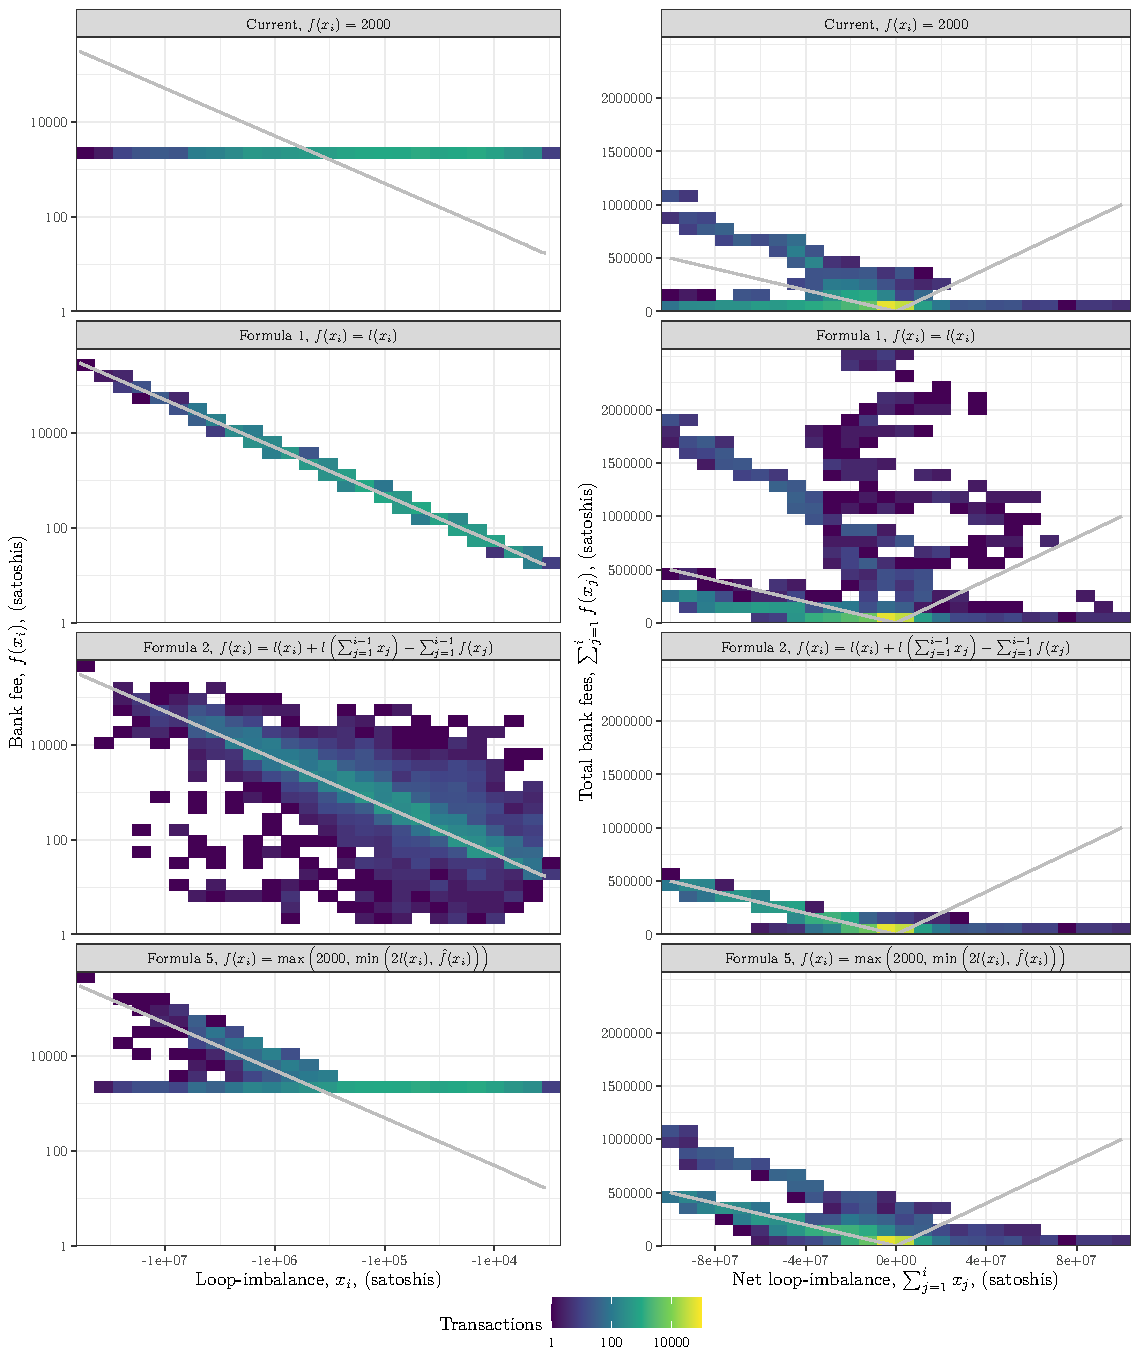
\includegraphics[width=\textwidth]{fig/replay/full}
	\caption[Fee structures]{ \label{sims}
		Fee structures applied to a historical dataset of transactions
		on the Bitcoin Beach Wallet during the second half of 2021.
		The left column shows the bank fee as a function of the loop imbalance
		created by the transaction under the different fee formulae.
		Only onchain payment transactions are shown, all other transactions
		are free except for protocol fees.
		The right column shows all onchain and offchain transactions
		plotted according to the initiating user's cumulative effect on loop imbalance
		at the time of the transaction.
		Plots on the right column are cropped to show a maximum
		loop imbalance of one bitcoin in either direction.
		Gray lines show the modeled market rate for loop imbalance correction, $l(\cdot)$.
		Transactions above the market rate lines,
		overpay for their individual effect on loop imbalance (left),
		or belong to users that have overpaid
		for their cumulative effect on loop imbalance (right).
	}
\end{figure*}

To understand how these different fee structures
may perform in a realistic usage context,
we analyzed a historical transaction dataset of
Bitcoin Beach Wallet users in the second half of 2021.
We replay the transactions under different fee structures
and calculate what the fees charged to users would have been,
and how that compares to the users' impact on loop imbalance.
In Figure~\ref{sims}
we plot two complimentary ways
of looking at the consequences of different fee structures:
(Left column) fees per transaction as function of the transaction's effect on  loop imbalance
(note the logarithmic scales), and
(Right column) cumulative fees collected per transaction
as a function of the user's net loop imbalance.
Gray lines on each panel allow us to contrast the
transaction fees collected with the modeled market rates for
loop imbalance correction.
When a user's transaction happens below these lines,
the user is creating an imbalance
that the bank may have to correct at its own expense.

Since fee structures will impact user behavior,
we must note that the predictive power of these transaction replay simulations
diminishes as the fee structures we simulate get further from
the fee structure that was in place when the transactions were made.
The Bitcoin Beach Wallet only charges a bank fee
above the protocol fee for onchain payments.
Thus, in our simulations, we applied fees according to
Formula~\ref{eq:simple} and Formula~\ref{eq:balancing}
only to onchain payments.
Furthermore, instead of using Formula~\ref{eq:cap},
we used a similarly intentioned, but less distant formula
in Figure~\ref{sims}:
\begin{equation} \label{eq:bbw}
	f(x_i) = \mathrm{max}\left( 2000,\,
		\mathrm{min}\left( \kappa l(x_i),\, \hat{f}(x_i) \right)\right)
\end{equation}
where, again, $\hat{f}$ is Formula~\ref{eq:balancing} above.

The first row of Figure~\ref{sims} shows the imbalance
fee structure currently implemented in the Bitcoin Beach Wallet:
a flat 2,000 satoshi bank fee on onchain payments.
The right column of that first row shows that
most users have a negative impact on the bank's loop imbalance
and that only a few pay the market rate to correct that imbalance.
The transactions above the market rate lines belong to users that overpay for their liquidity imbalance,
making many onchain payments while maintaining a low net imbalance.
The transactions below the market rate lines belong to users that underpay for their liquidity imbalance,
receiving large amounts of bitcoin offchain but only rarely paying onchain.

Comparing the different fee formulae proposed here,
we see that only the self-balancing formulae
have the effect of keeping most transactions
at or above the market rate lines.
As expected,
the simplest self-balancing formula, Formula~\ref{eq:balancing},
does the best job at charging users exactly as much fees
as the imbalance they create costs.
However, we can see that the simple self-balancing
Formula~\ref{eq:balancing}  has significantly more variable fees than
the naive Formula~\ref{eq:simple}.
The self-balancing fee structure
described in Formula~\ref{eq:bbw},
appears to have a good balance of predictability and proper pricing
even when applied only to onchain payments.
This fee structure,
with maximum fee rate limited to twice the market rate,
would result in a flat fees for 98\% of onchain payments and
allow 94\% of users to only ever be charged a flat fee.

\section{Discussion}

This work was motivated by the discovery that
a few users of the Bitcoin Beach Wallet
were using the wallet as a fee-efficient way of
acquiring additional inbound liquidity.
This activity had the effect of consistently reducing the bank's
onchain liquidity and offchain inbound liquidity.
The problem was made worse by the fact that the Bitcoin Beach Wallet,
operates with significant constraints on total liquidity
because most reserves are kept illiquid, in cold storage.
To the extent that the bank's ability to process transactions for its users was affected,
it was necessary to pay for a swap service to
restore onchain liquidity and inbound liquidity.
The current market rate for inbound liquidity on the Lightning network is not trivial.
Although, protocol developments like splicing
and PeerSwap will reduce some of the costs associated with
acquiring additional inbound liquidity,
the cost of inbound capital allocation is likely to remain significant.

We described several fee structures that account for each user's impact
on the bank's onchain and offchain liquidity balance.
Since these fee structures assure that the fees paid by a user
asymptotically approach the market cost of inbound liquidity,
their implementation will remove the opportunity of arbitrage.
We verified through a simulation study,
that formulae that keep track of a user's net
contribution to imbalance between onchain and offchain liquidity
and total fees paid, do a good job of charging users appropriate fees
in realistic scenarios.
And we showed that limiting these self-balancing fee structures
can ensure a relatively simple user experience.

Finally, the fee structures discussed here
may have applications outside of custodial Bitcoin banks.
Non-custodial Lightning wallets like
Phoenix\footnote{\url{https://phoenix.acinq.co/}} and
Breez\footnote{\url{https://breez.technology/}},
use submarine swap services to enable their users to participate in onchain transactions.
This is equivalent to a custodial wallet using the fee structure
described in Formula~\ref{eq:simple}.
The fee structures described here could be used by a new
submarine swap service to sustainably reduce the fee
burden of everyday non-custodial Lightning wallet users.

\section*{Acknowledgments}

We thank Alex Bosworth for helpful comments on
a previous draft of this manuscript
and Christian Decker for providing an updated version
of the Lightning network gossip message archive \citep{lngossip}.

\bibliography{references}

\end{document}
